% 波的强度

\pentry{波的能量\upref{WaEner}}

为了描述能量随着波动的进行而在介质中传播的情况,引入能流的概念.

单位时间内通过介质中某面积的能量称为通过该面积的\textbf{能流}(energy flow).设在某一介质中,垂直于波速$u$的方向,取面积$S$,则在单位时间内通过$S$面的能量等于体积$uS$中的能量,如\autoref{WaInte_fig1}所示
\begin{figure}[ht]
\centering
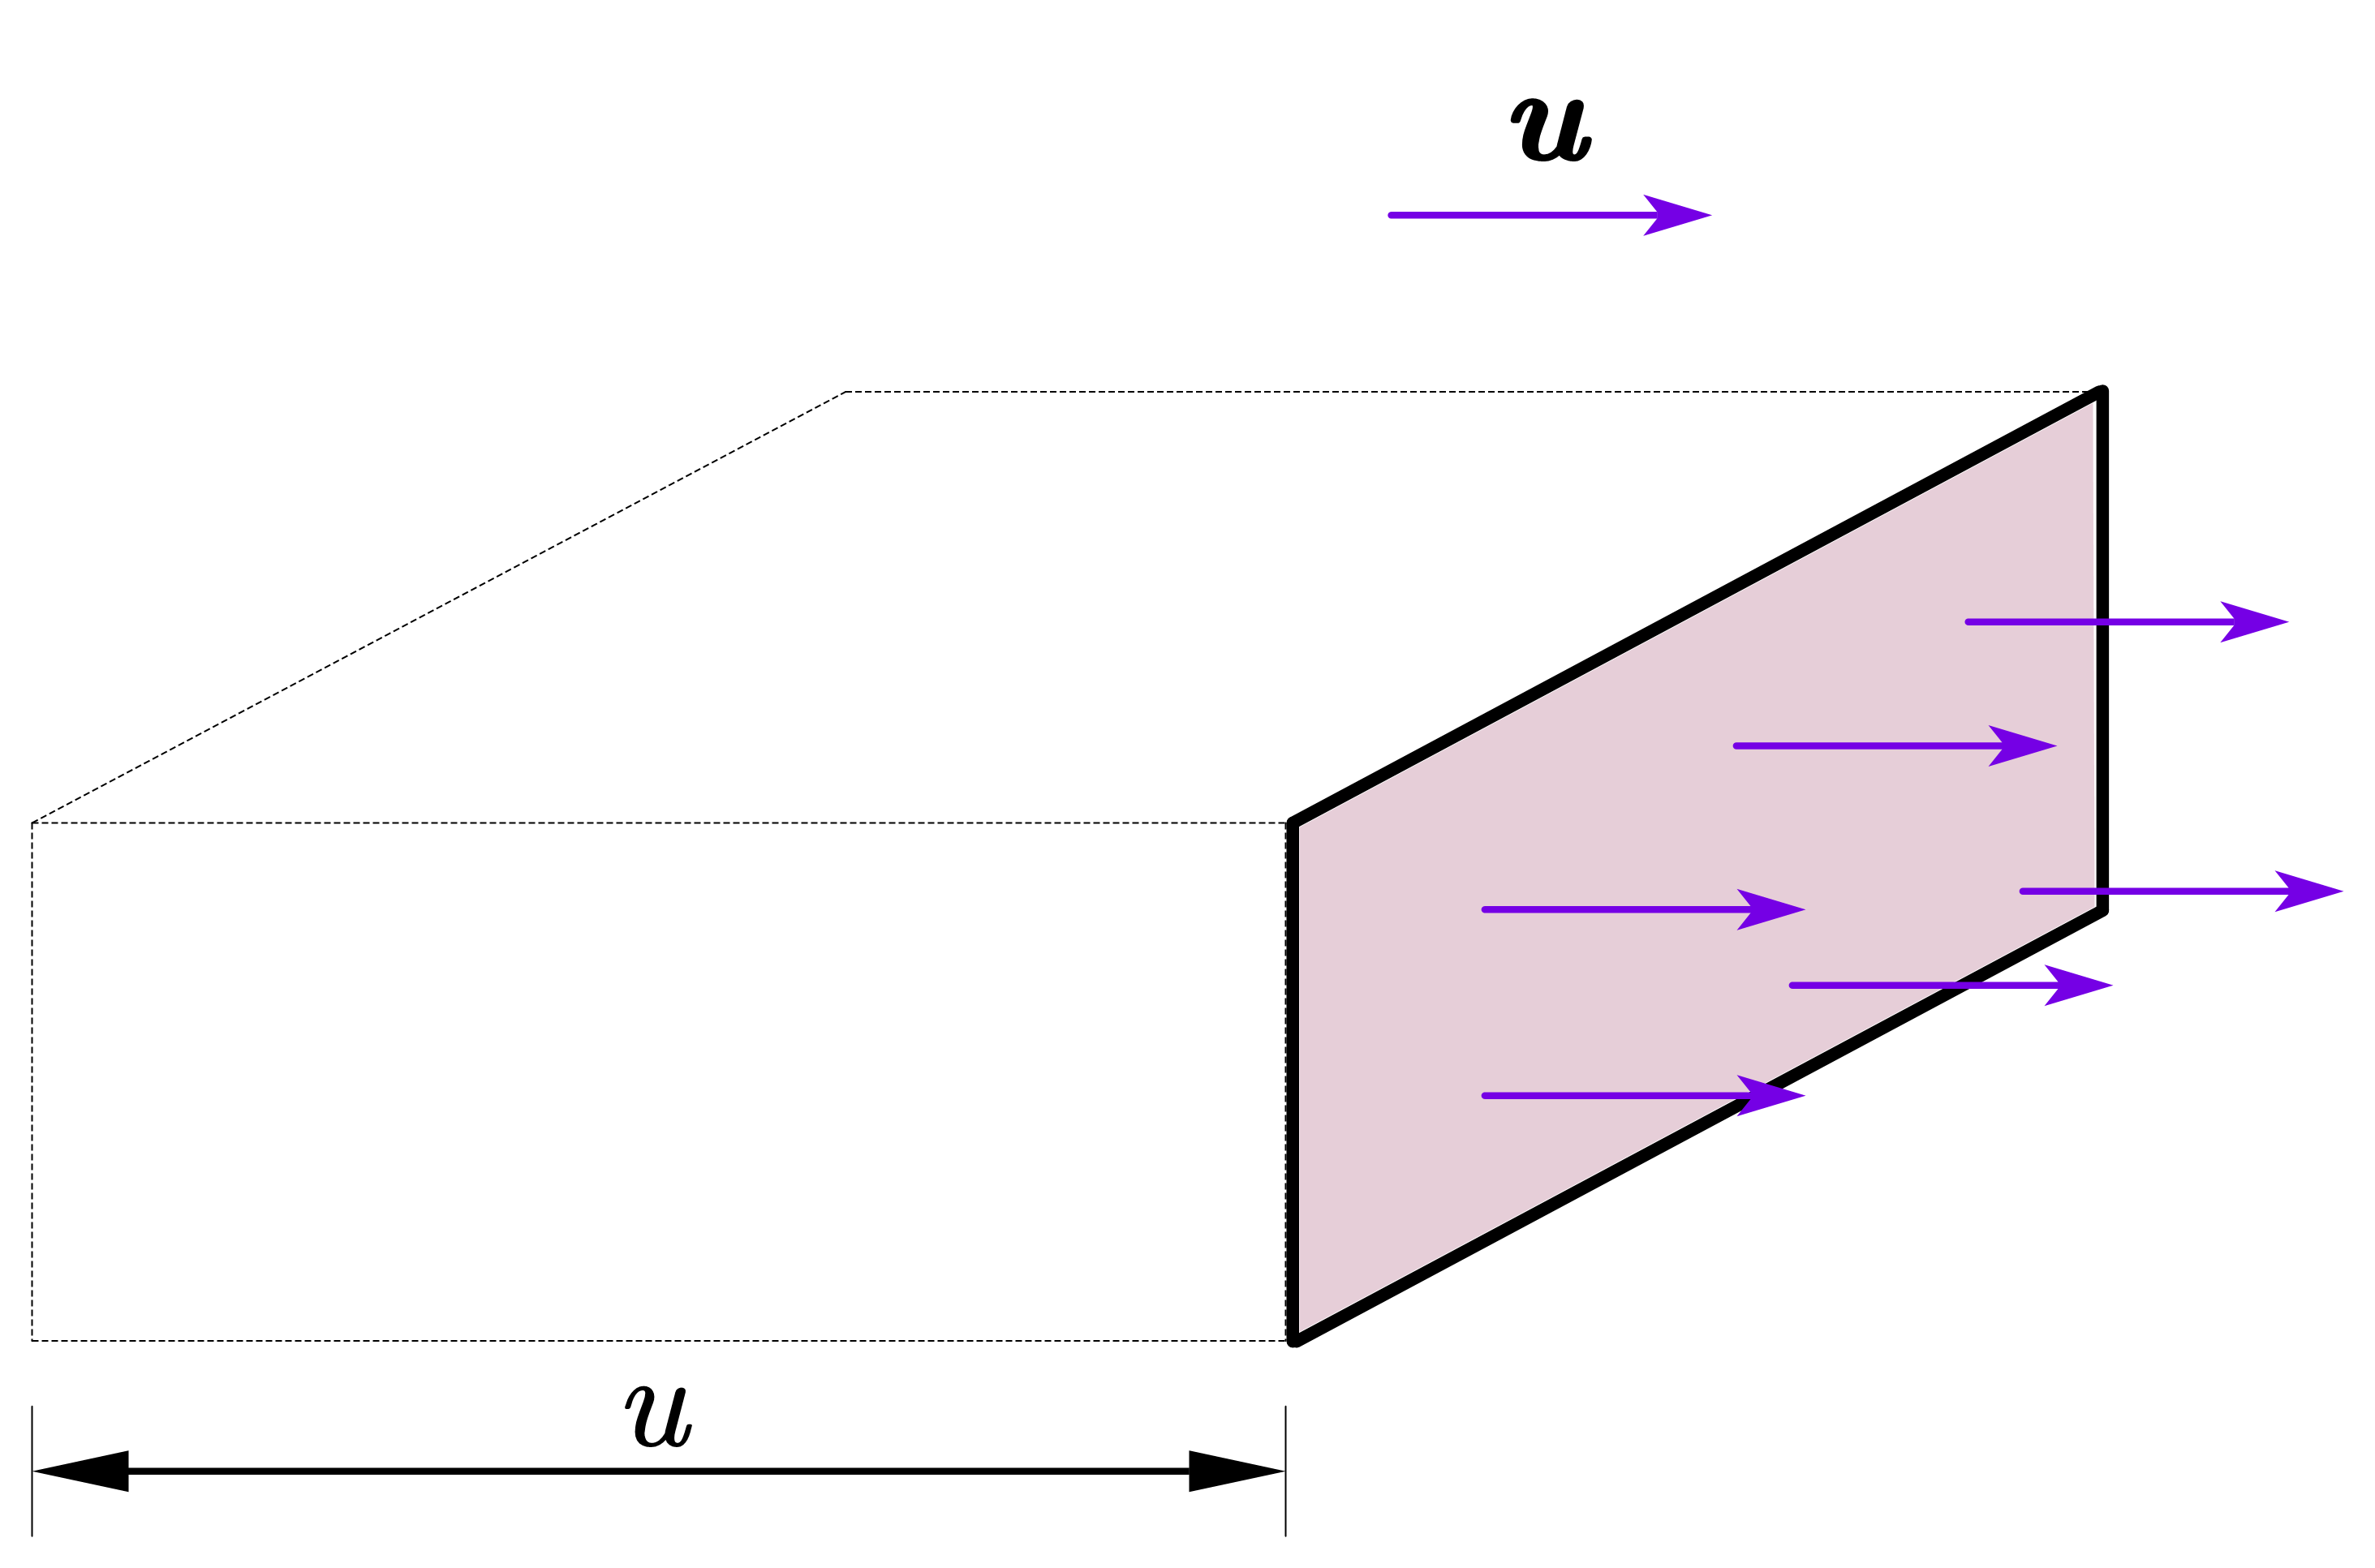
\includegraphics[width=7cm]{./figures/WaInte_1.png}
\caption{体积$uS$内的能量在单位时间内通过$S$面} \label{WaInte_fig1}
\end{figure}

此能量是周期性变化的,通常取其一个周期的时间平均值,得到平均能流为
\begin{equation}
\overline{P}=\overline{w} u S
\end{equation}
式中,$\overline w$为平均能量密度.通过与波动传播方向垂直的单位面积的平均能流,称为\textbf{平均能流密度},又称\textbf{波的强度}(intensity of wave),用$I$来表示,即
\begin{equation} \label{WaInte_eq1}
I=\overline{w} u=\frac{1}{2} \rho u \omega^{2} A^{2}=\frac{1}{2} Z \omega^{2} A^{2}
\end{equation}
其中
\begin{equation}
Z=\rho u
\end{equation}
是表征介质特性的一个常量,称为介质的\textbf{特性阻抗}.\autoref{WaInte_eq1}表明,弹性介质中简谐波的强度正比于振幅的平方,正比角频率(或频率)的平方,还正比于介质的特性阻抗.在国际单位制中,波的强度单位为$\mathrm{W}/\mathrm{m^2}$.